\documentclass{article}
\usepackage[utf8]{inputenc}
\usepackage[T1]{fontenc}
\usepackage{amsmath}
\usepackage{graphicx}
\usepackage{listings}
\usepackage{xcolor}
\usepackage{makecell}
\usepackage{float}

\lstset{
	language=C++,
	backgroundcolor=\color{black!5},
	basicstyle=\footnotesize\ttfamily,
	keywordstyle=\color{blue},
	commentstyle=\color{green!50!black},
	stringstyle=\color{red!70!black},
	numbers=left,
	numberstyle=\tiny\color{gray},
	stepnumber=1,
	frame=single,
	rulecolor=\color{black!30},
	tabsize=4,
	breaklines=true,
	breakatwhitespace=false,
	showspaces=false,
	showstringspaces=false,
	showtabs=false
}

\title{Analiza i porównanie algorytmów CUT\_ROD, LCS i ACTIVITY\_SELECTOR}
\author{Tomasz Warzecha}

\begin{document}
	
	\maketitle
	
	\section{Wstęp}
	W sprawozdaniu moim celem jest analiza i porównanie wydajności trzech algorytmów: CUT\_ROD, LCS oraz ACTIVITY\_SELECTOR. Algorytmy te zostały zaimplementowane w różnych wersjach: rekurencyjnej, ze spamiętywaniem oraz iteracyjnej. Dodatkowo w ACTIVITY\_SELECTOR został zmodyfikowany w taki sposób aby działał na danych wejściowych posortowanych względem czasu rozpoczęcia, nie zakończenia. Niektóre z algorytmów również posiadają funkcje odzyskiwania rozwiązań. Badania skupiają się na porównaniu teoretycznych złożoności czasowych oraz praktycznych czasów wykonania dla różnych rozmiarów danych.
	
	\section{Implementacja algorytmów}
	Algorytmy zostały zaimplementowane zgodnie z klasycznymi wersjami, z uwzględnieniem modyfikacji wskazanych w poleceniach.
	
	\paragraph{Najciekawsze fragmenty kodu\\}
	Poniżej przedstawię najciekawsze fragmenty kodu, wraz z objaśnieniami, tak aby łatwiej zrozumieć działanie algorytmów.
	
	\subsection{\textit{CUT\_ROD}}
	W algorytmie CUT\_ROD wersja ze spamiętywaniem wykorzystuje tablicę do przechowywania wyników pośrednich, co znacznie redukuje złożoność czasową. Poniżej przedstawiono kluczowy fragment kodu, który wraz z fragmentem zapisującym wynik dla danego n w naszej tablicy tworzy główne usprawnienie naiwnego algorytmu:
	\newpage
	\begin{lstlisting}
if (R[n-1]>=0){
	return R[n-1];
}
	\end{lstlisting}
	Ten fragment sprawdza, czy wynik dla danego `n` został już obliczony i zapisany w tablicy `R`. Jeśli tak, zwraca zapisaną wartość, unikając ponownego obliczania.
	
	\subsection{\textit{LCS}}
	W algorytmie LCS wersja iteracyjna wykorzystuje dwie tablice do przechowywania długości najdłuższego wspólnego podciągu oraz kierunku, w którym należy się poruszać, aby odtworzyć rozwiązanie. Poniżej znajduje się kluczowy fragment kodu:
	
	\begin{lstlisting}
if (X[i-1] == Y[j-1]) {
	C[i][j] = C[i-1][j-1] + 1;
	B[i][j] = '-';
}
	\end{lstlisting}
	Ten fragment sprawdza, czy znaki w obu ciągach są takie same. Jeśli tak, zwiększa długość najdłuższego wspólnego podciągu i zapisuje kierunek w tablicy `B`.
	
	\subsection{\textit{ACTIVITY\_SELECTOR}}
	W algorytmie ACTIVITY\_SELECTOR wersja dynamiczna wykorzystuje dwie tablice do przechowywania liczby zajęć oraz indeksów zajęć, które należy wybrać. Poniżej przedstawiono kluczowy fragment kodu:
	
	\begin{lstlisting}
while (f[i] < f[k]) {
	if (f[i] <= s[k] && f[k] <= s[j] && c[i][k]+c[k][j]+1> c[i][j]) {
		c[i][j] = c[i][k]+c[k][j]+1;
		act[i][j] = k;
	}
	k--;
}
	\end{lstlisting}
	Ten fragment sprawdza, czy zajęcia się nie nakładają i czy wybór danego zajęcia zwiększa liczbę możliwych do wybrania zajęć. Jeśli tak, aktualizuje tablice `c` i `act`, tak aby zawierała aktualnie najwiekszą ilość zadań między dwoma indeksami.
	\newpage
	\section{Porównanie algorytmów}
	
	\subsection{Porównanie teoretyczne}
	Poniżej zestawiono złożoności czasowe oraz pamięciowe dla różnych wersji algorytmów:
	
	\begin{table}[H]
		\begin{tabular}{|l|c|c|c|}
			\hline
			\textbf{Algorytm} & \textbf{Rekurencyjna} & \textbf{Spamiętywanie} & \textbf{Iteracyjna} \\ \hline
			\textit{CUT\_ROD} & $O(2^n)$ & $O(n^2)$ & $O(n^2)$ \\ \hline
			\textit{LCS} & $O(2^{m+n})$ & $O(mn)$ & $O(mn)$ \\ \hline
			\textit{ACTIVITY\_SELECTOR} & $O(n)$ & - & $O(n)$ \\ \hline
		\end{tabular}
		\caption{Porównanie teoretyczne algorytmów}
	\end{table}
	
	\subsection{Porównanie czasów działania}
	Zaprezentowano wyniki pomiarów na wykresach:
	
	\begin{figure}[H]
		\centering
		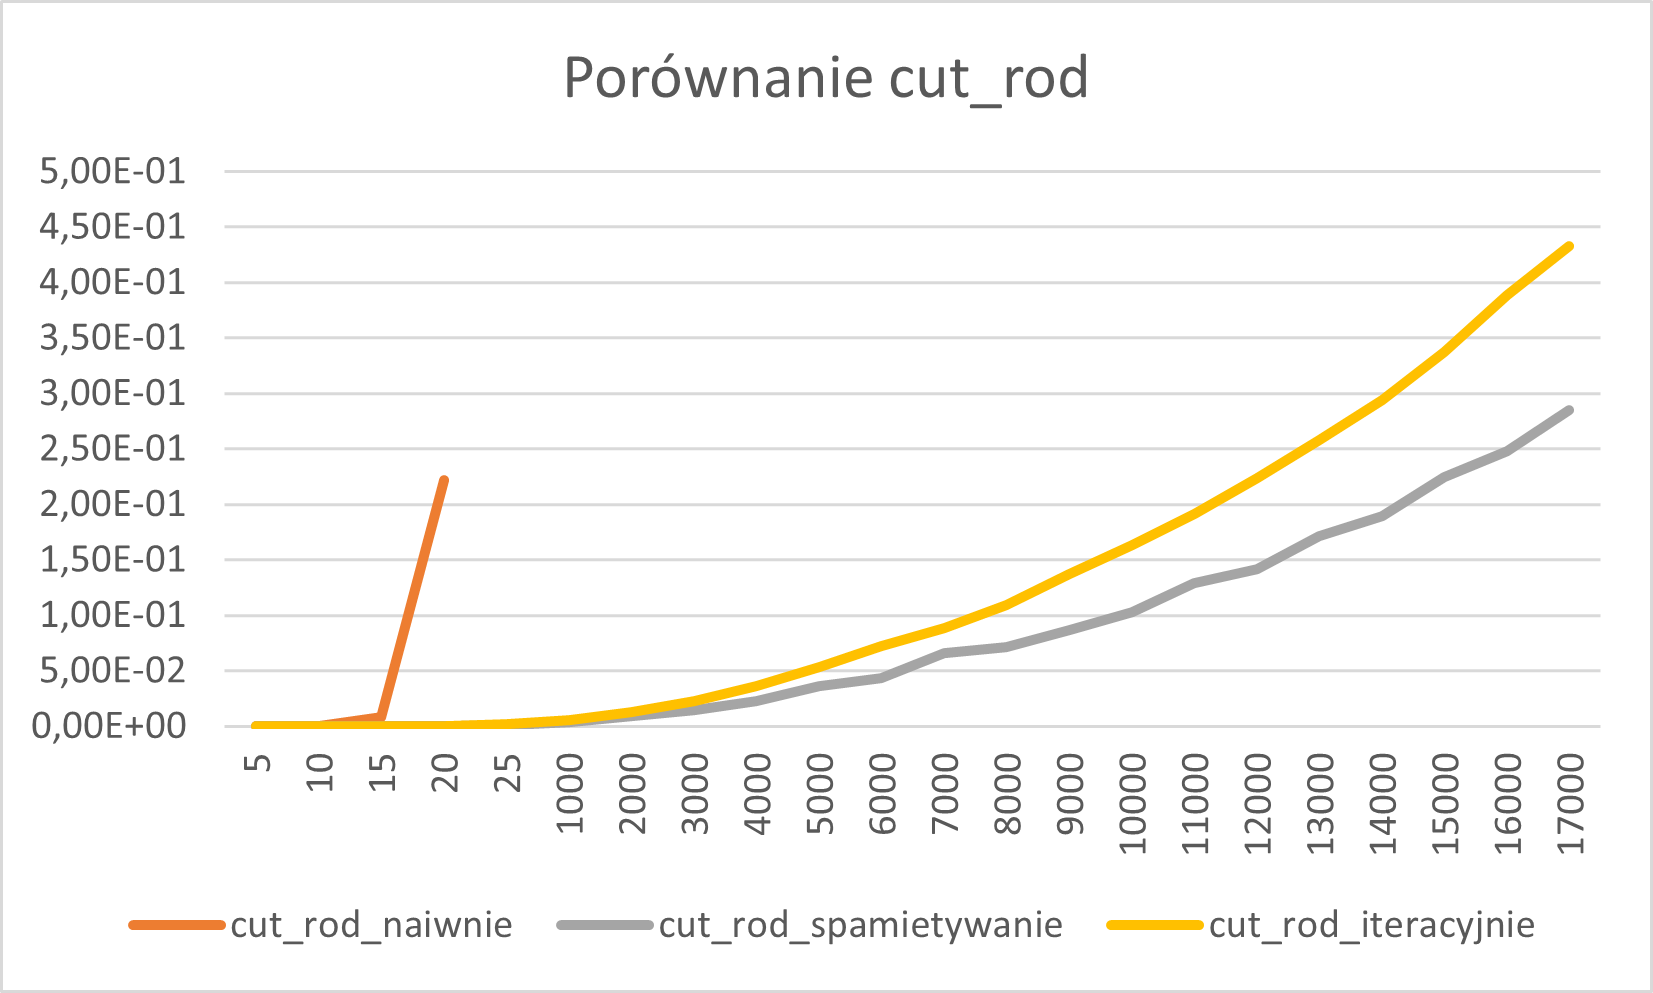
\includegraphics[width=\textwidth]{cut_rod.png}
		\caption{Porównanie czasów działania \textit{CUT\_ROD} w różnych wersjach.}
	\end{figure}
	 Łatwo możemy zauważyć na wykresie, że naiwna wersja CUT\_ROD jest bardzo czasochłonna. Jest to spowodowane wykładniczą złożonością czasową, podczas gdy wersje ze spamiętywaniem i iteracyjna mają złożoność kwadratową. Zatem dwie ostatnie wersje są znacząco szybsze i podobne czasowo do siebie.
	\begin{figure}[H]
		\centering
		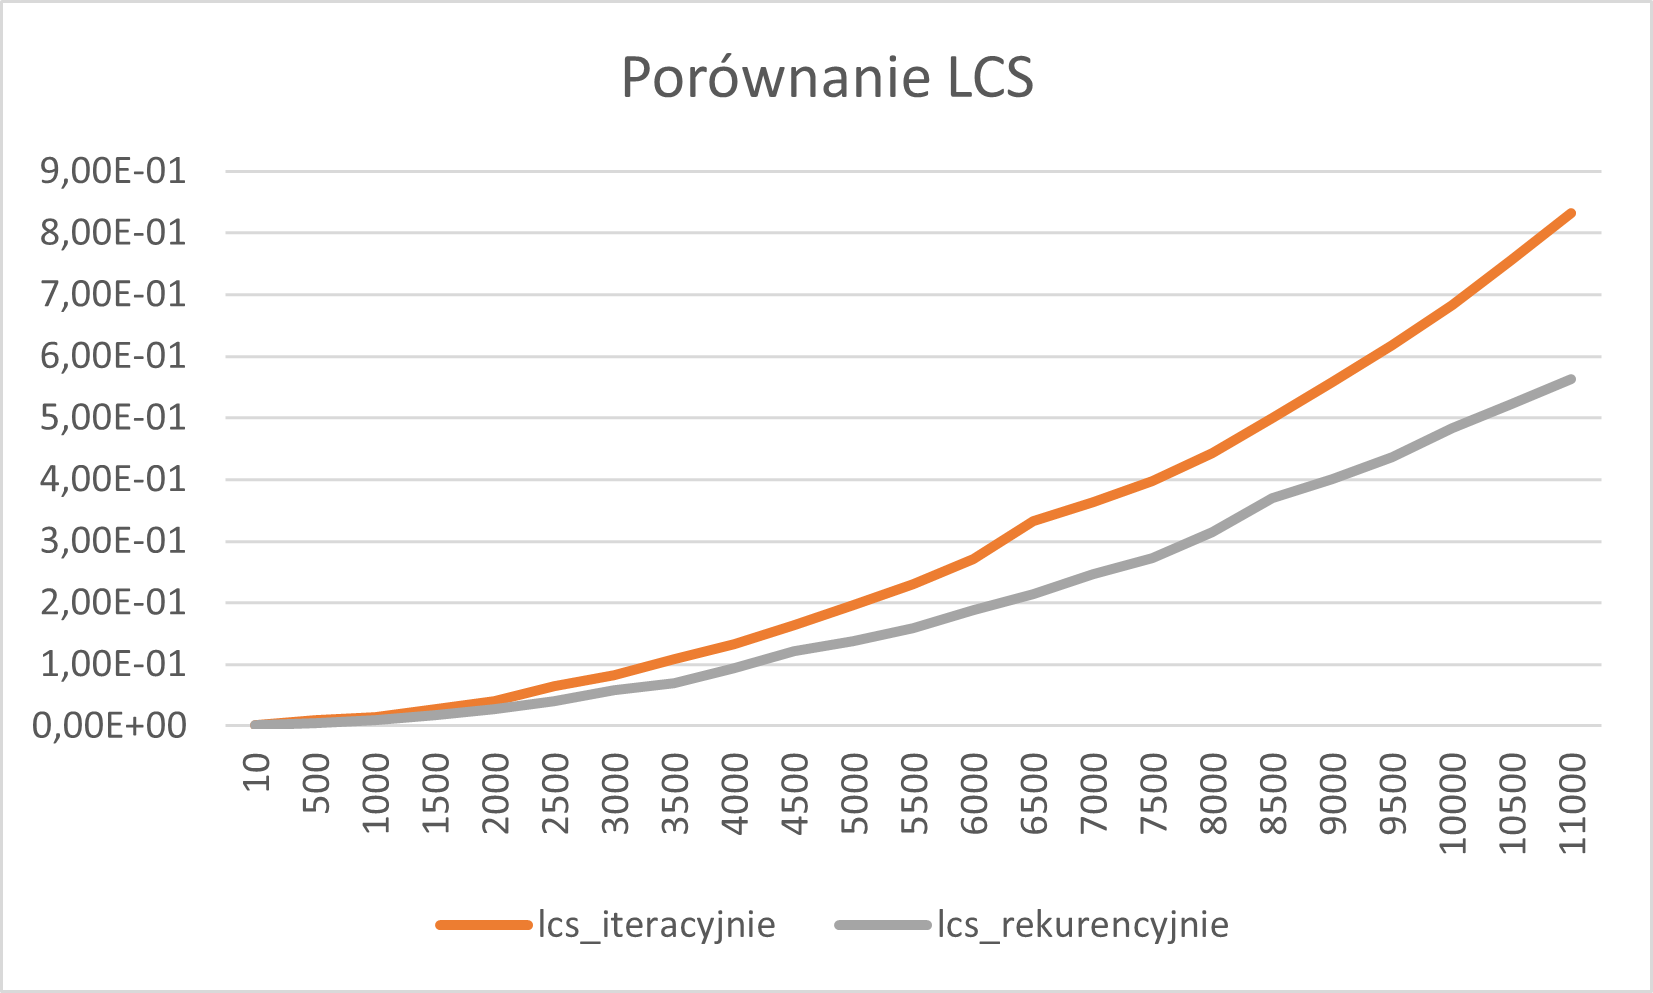
\includegraphics[width=\textwidth]{lcs.png}
		\caption{Porównanie czasów działania \textit{LCS} w różnych wersjach.}
	\end{figure}
	 Możemy zauważyć że czas wykonania lcs w wersji iteracyjnej i rekurencyjnej jest podobny, różnice są niewielkie. Jest to spowodowane taką samą złożonością algorytmów - $n^2$.
	\begin{figure}[H]
		\centering
		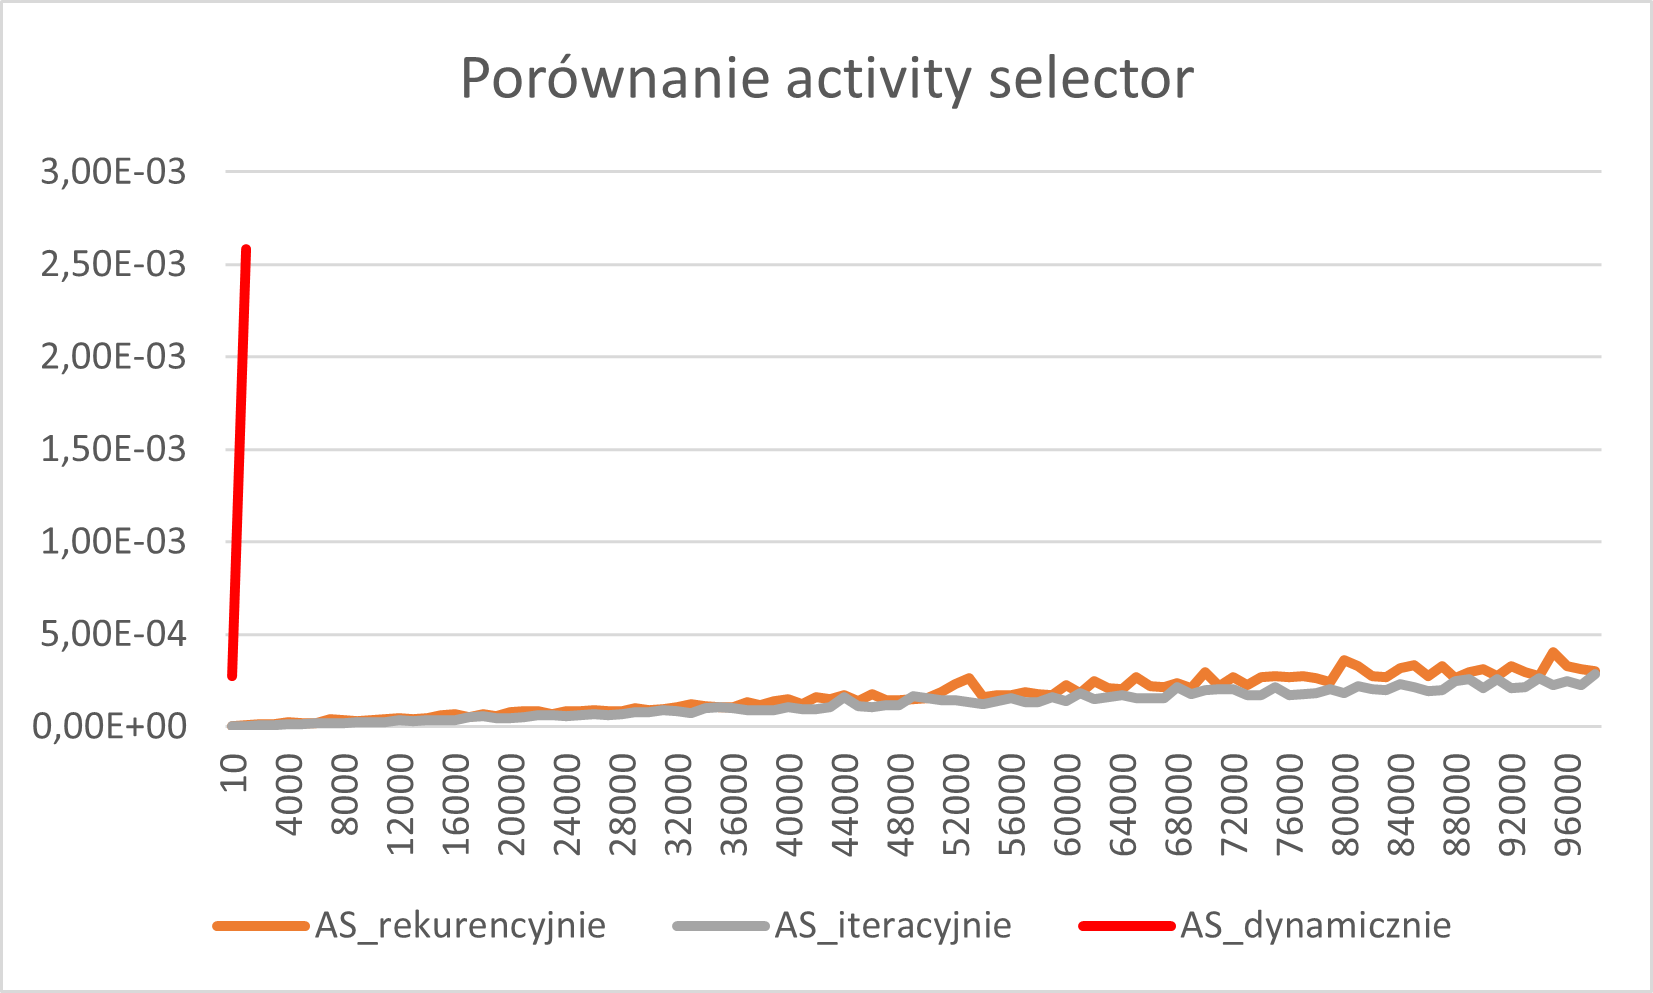
\includegraphics[width=\textwidth]{as.png}
		\caption{Porównanie czasów działania \textit{ACTIVITY\_SELECTOR} w różnych wersjach.}
	\end{figure}
	 Jak możemy zauważyć, dynamiczna wersja AS ma dużo większą złożoność czasową, ponieważ aż $n^3$, co od razu widać na rysunku. Wersje rekurencyjna i iteracyjna mają złożoność liniową i nieznacznie się od siebie różnią.
	\section{Porównanie modyfikacji}
	
	\subsection{\textit{ACTIVITY\_SELECTOR}}
	Zmodyfikowana wersja algorytmu ACTIVITY\_SELECTOR działa na danych posortowanych względem czasu rozpoczęcia. Poniżej przedstawiono wyniki porównania czasów działania:
	
	\begin{figure}[H]
		\centering
		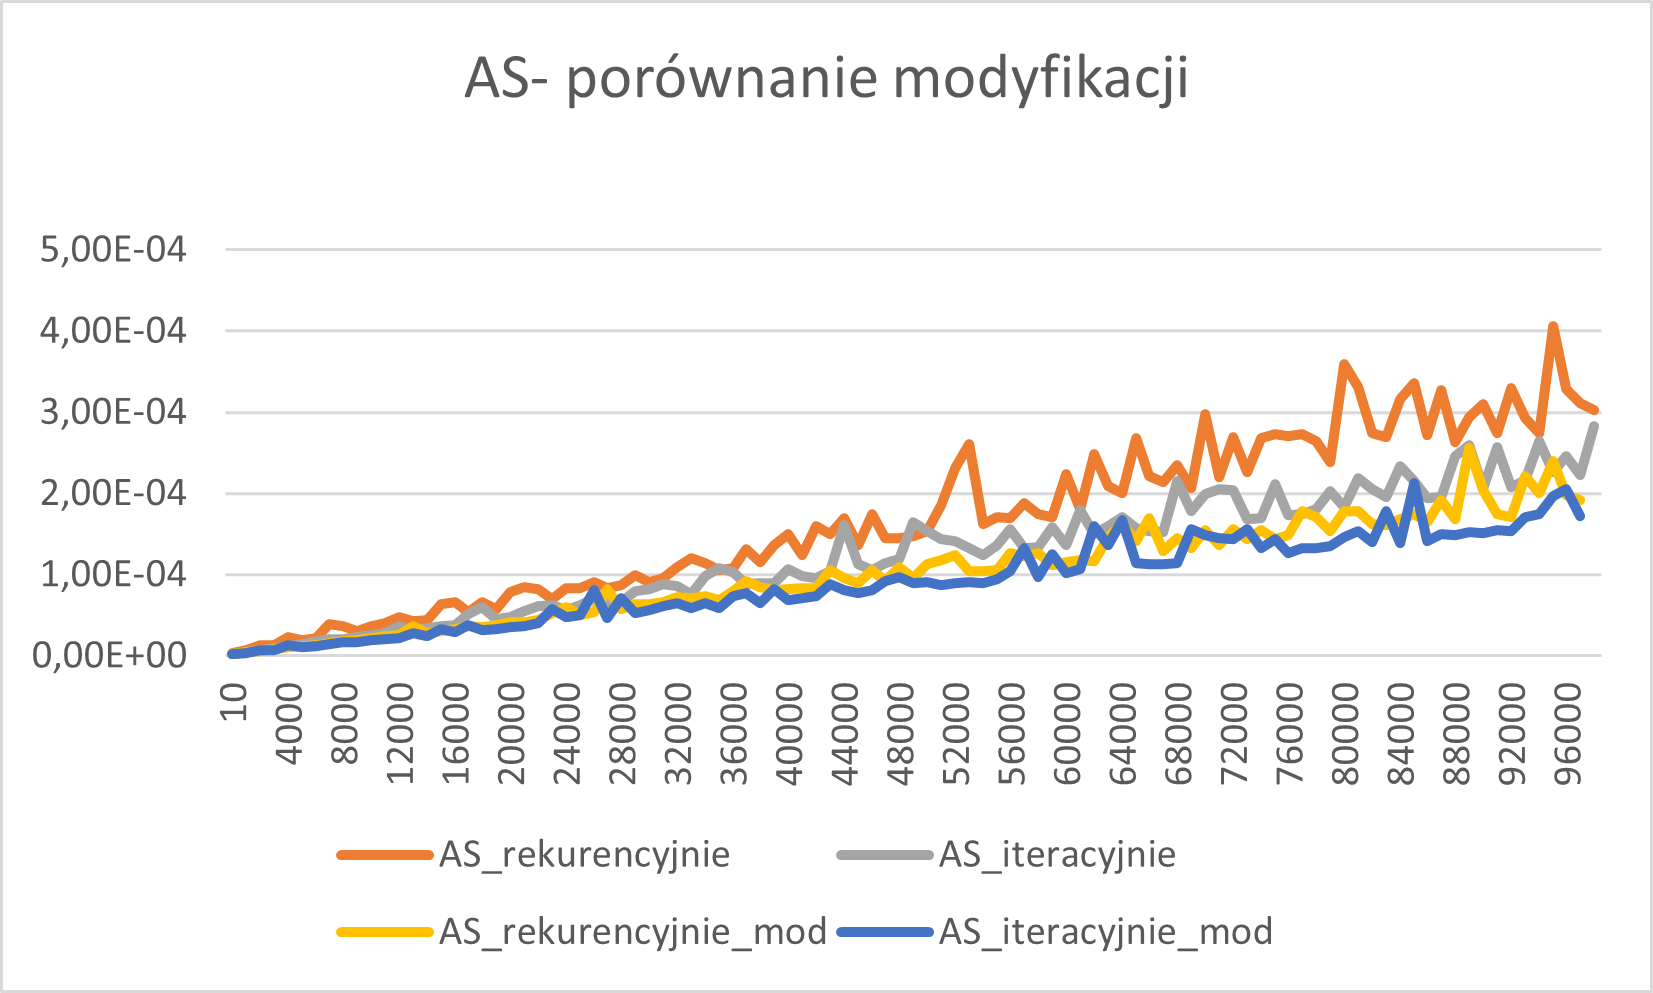
\includegraphics[width=\textwidth]{as_mod.png}
		\caption{Porównanie czasów działania \textit{ACTIVITY\_SELECTOR} i jego modyfikacji.}
	\end{figure}
	Modyfikacja algorytmu polegała na otrzymywaniu danych wejściowych posortowanych względem czasu rozpoczęcia zamiast zakończenia. Na wykresie możemy zobaczyć, że niezależnie od tego czy mamy posortowane czasy rozpoczęcia, czy zakończenia czas działania pozostaje na podobnym poziomie, delikatne różnice mogą wynikać z różnego obciążenia komputera podczas testów. 
	\newpage
	\section{Wnioski}
	Przeprowadzone testy pokazują, że wersje algorytmów ze spamiętywaniem oraz iteracyjne są w większości przypadków znacznie bardziej wydajne niż ich rekurencyjne odpowiedniki. Jedynie w przypadku ACTIVITY\_SELECTOR wersja rekurencyjna jest na tym samym poziomie, jednak wynika to z istoty problemu. Modyfikacje algorytmów nie wpływają znacząco na poprawę wydajności oraz powodują większe skomplikowanie kodu, zatem nie warto z nich korzystać.
	
\end{document}